\documentclass[xcolor={dvipsnames},pdf, hyperref={colorlinks=true, citecolor=ForestGreen, linkcolor=BlueViolet, urlcolor=Magenta}]{beamer}
\usetheme{Frankfurt}  
\usecolortheme{whale}
\usepackage{tikz} 
\usepackage{graphicx}
\usepackage{dsfont}
\usepackage{hyperref}
\usepackage{alltt}
\usepackage{enumerate}
\usepackage{amsthm}
\theoremstyle{definition}
\newtheorem{exmp}{Example}[section]
\usepackage{verbatim}               % useful for \begin{comment} and \end{comment}
\usepackage{eurosym}                % used for euro symbol
\usepackage{caption} 
\usepackage{graphicx}
\usepackage{adjustbox}
\graphicspath{{Figures/}}
\usepackage{subcaption}
\usepackage{color}
\usepackage{float}
\usepackage{amssymb}
\usepackage{sgamevar}
\usepackage{remreset}% tiny package containing just the \@removefromreset command
\makeatletter
\@removefromreset{subsection}{section}
\makeatother
\setcounter{subsection}{1}


\newcommand{\defn}[1]{\textbf{#1}}


%Instructor version
\newcommand{\blank}[0]{}
\newcommand{\ddp}[1]{{\textcolor{ForestGreen}{#1}}} 
\newcommand{\dd}[1]{{\underline{\textcolor{ForestGreen}{#1}}}}

%Student version
%\newcommand{\blank}[0]{\vspace{2em}}
%\newcommand{\dd}[1]{\underline{\hspace{3cm}}} 
%\newcommand{\ddp}[1]{}

\addtobeamertemplate{navigation symbols}{}{%
	\usebeamerfont{footline}%
	\usebeamercolor[fg]{footline}%
	\hspace{1em}%
	\insertframenumber/\inserttotalframenumber
}

\section{Model Assumptions}

%% preamble
\title{The Solow Model}
\author{David A. D\'iaz}
\institute{UNC Chapel Hill}
\date{}

\AtBeginSection[] %Section links on slides

\begin{document} 
	
	\begin{frame}
		
		\titlepage
		
	\end{frame}


\begin{frame}{The Solow Model}
\begin{itemize}
	\item \defn{Production Function:} A function that describes the relationship between the quantity of inputs used in production and the quantity of output.
	\item We will assume that real GDP ($Y$) is a function of \dd{capital}, \dd{labor}, and \dd{technology}. 
	\item Thus, we can write $Y = A\cdot F(K,L)$, where $A$ reflects the available production technology and is a measure of productivity.
\end{itemize}
\end{frame}

\begin{frame}{The Solow Model}
\begin{itemize}
	\item Assumptions:
\begin{enumerate}
	\item Increasing returns to inputs: More $K$ or $L$ leads to greater $Y$.
	\item Diminishing marginal returns: As $K$ or $L$ increase, their marginal product decreases.
	\item Constant returns to scale: $F(\lambda K, \lambda L) = \lambda F(K,L)$.
\end{enumerate}

\end{itemize}
\end{frame}

\begin{frame}{The Solow Model}
\begin{itemize}	
	\item For now, we will assume that technology and labor are constant so that we can write our production function as $Y = F(K)$.
	\item Using the property of \dd{constant returns}, we can write the output per worker, or real GDP per capita, as 
	\[y = Y/L = 1/L \cdot F(K,L) = F(K/L,L/L) = F(K/L) \equiv f(k) \]
	where $k \equiv K/L$ is the capital-labor ratio.
\end{itemize}
\end{frame}

\begin{frame}{The Solow Model}
\begin{exmp} 
	Suppose output per worker in an economy is described by $y = \sqrt{k}$. If each worker has 100 units of capital, how much output can each produce? What if each had 200 units? 300? What property does this production function exhibit?
\end{exmp}
\ddp{\pause $y = \sqrt{100} = 10$ \\ 
\pause	$y = \sqrt{200} = 14.14$ \\
\pause	$y = \sqrt{300} = 17.32$}
\end{frame}

\begin{frame}{The Solow Model}


	\begin{figure}[H]
		\centering
		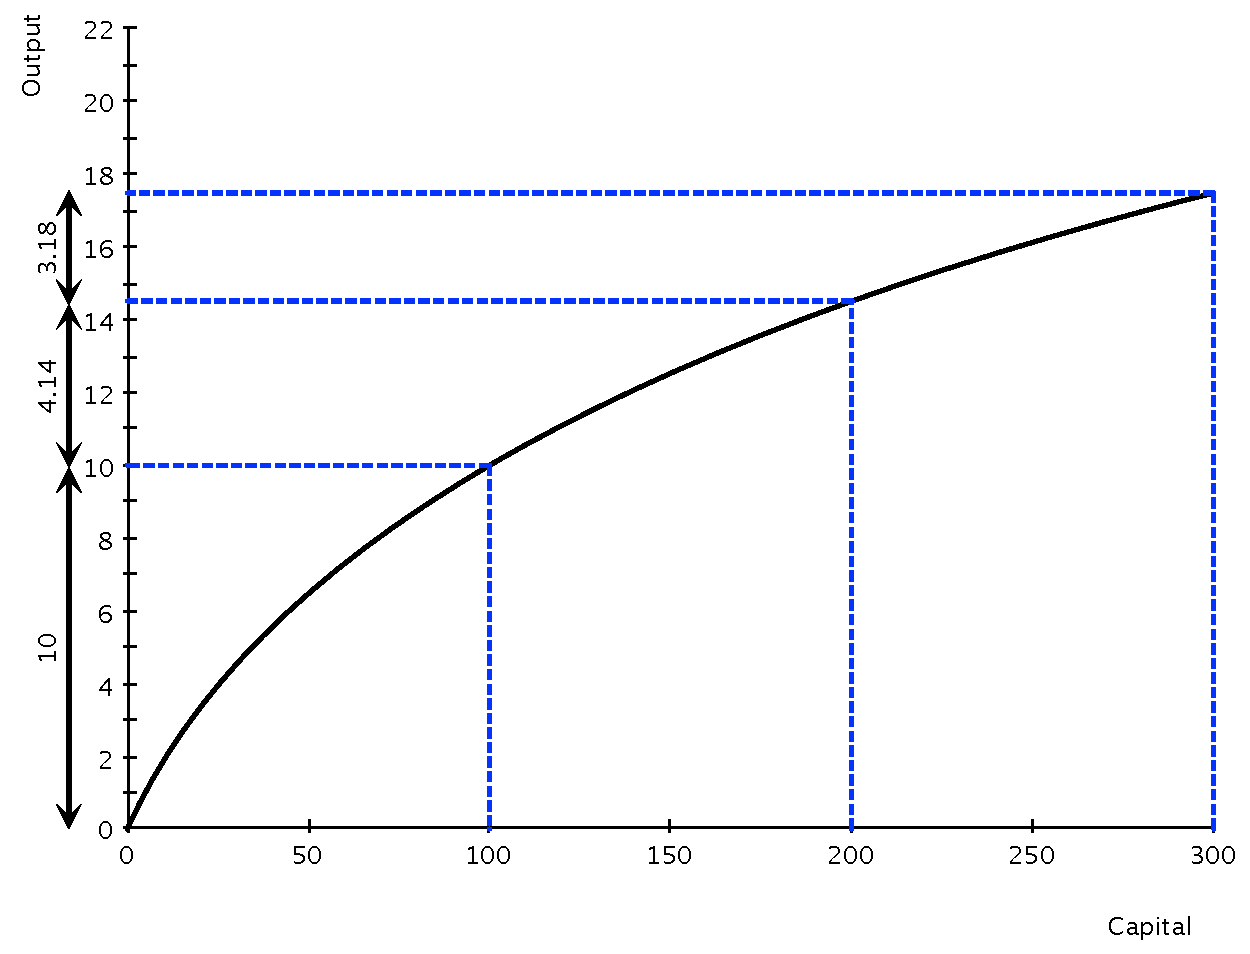
\includegraphics[scale=.35]{plot83.pdf}
		\caption{Returns to Capital}
\end{figure}

\end{frame}

\begin{frame}{The Solow Model}
\begin{exmp}
	The United States and China both have this same production function. However, the US currently has 400 units of capital per worker, while China only has 225. If both countries receive another 100 units of capital worker this year, what will be the growth rate of real GDP per capita in each country? 
\end{exmp}
\ddp{$y_0^{us} = \sqrt{400} = 20$. \\
	\pause $y_1^{us} = \sqrt{500} = 22.36$ \\
	\pause $\hat{y}^{us} = (22.36-20)/20 \times 100\% = 11.8\%.$ \\ 
\pause	$y_0^{china} = \sqrt{225} = 15$ \\
\pause $y_1^{china} = \sqrt{325} = 18.03$ \\
\pause $\hat{y}^{us} = (18.03-15)/15 \times 100\% = 20.2\%.$} 

\end{frame}

\begin{frame}{The Solow Model}

\begin{itemize}
	\item Due to diminishing returns, countries with small capital stocks grow more rapidly than those with large capital stocks. However, as capital accumulates, growth slows. 
\end{itemize}
\end{frame}

\section{Capital Accumulation}

\begin{frame}{The Solow Model}
\begin{itemize}
	\item We will assume that output can be used in one of two ways: 
	\begin{enumerate}
		\item Investment - used to produce more capital goods
		\item Consumption
	\end{enumerate}
	\item We assume that individuals save and invest a constant fraction of output, so we can write investment per worker in period $t$ as \dd{$i = sy$}, where $s$ is the savings rate.
	\item Since output is either invested or consumed, we can write the consumption per worker in the economy in time $t$ as \dd{$c = y - i = y - sy = (1-s)y$}.
\end{itemize}
\end{frame}

\begin{frame}{The Solow Model}
\begin{itemize}
	\item Each period, we assume a constant fraction of the initial capital stock depreciates and is unusable in the next period.
	\item Capital depreciation per worker in time $t$ is given as \dd{$d =\delta k$}, where $\delta$ is the depreciation rate.
	\item Finally, we can write the \textbf{law of motion} for capital per worker as \[k_{t+1} = k_t + i_t - d_t\]
\end{itemize}
\end{frame}

\begin{frame}{The Solow Model}
\begin{exmp} 
	A country has the production function $y = \sqrt{k}$ and an initial capital stock per worker of $k_0 = 25$. Assume capital depreciates 5\% every period and the country invests 20\% of their output for next period. How much output will they produce this period? How much will they invest? What will be the level of the capital stock, output, and real per capita GDP growth in the next three periods?
\end{exmp}
\begin{table}[ht]
	\centering
	\begin{tabular}{c|c|c|c|c|c}        
		
		$t$ & $k_t$ & $y_t = \sqrt{k_t}$ & $d_t = .05k_t$ & $i_t = .20y_t$ & $\hat{y}_t$ \\
		\hline
		0 & 25 & \ddp{5} & \ddp{1.250} & \ddp{1} & \ddp{---} \\
		1 & \ddp{24.750} & \ddp{4.975} & \ddp{1.238} & \ddp{.995} & \ddp{--.501\%}\\
		2 & \ddp{24.507} & \ddp{4.951} & \ddp{1.225} & \ddp{.990} & \ddp{--.491\%}\\
		3 & \ddp{24.272} & \ddp{4.927} & \ddp{1.214} & \ddp{.985} & \ddp{--.481\%} \\
		
	\end{tabular}
\end{table}
\end{frame}

\begin{frame}{The Solow Model}
\begin{itemize}
	\item When depreciation is \dd{greater} than investment, the capital stock is \dd{diminishing}. Thus, output is also \dd{decreasing}.
	\item Conversely, when depreciation is \dd{lower} than investment, the capital stock and output are both \dd{increasing}.
\end{itemize}
\end{frame}

\begin{frame}{The Solow Model}
\begin{figure}[H]
	\centering
	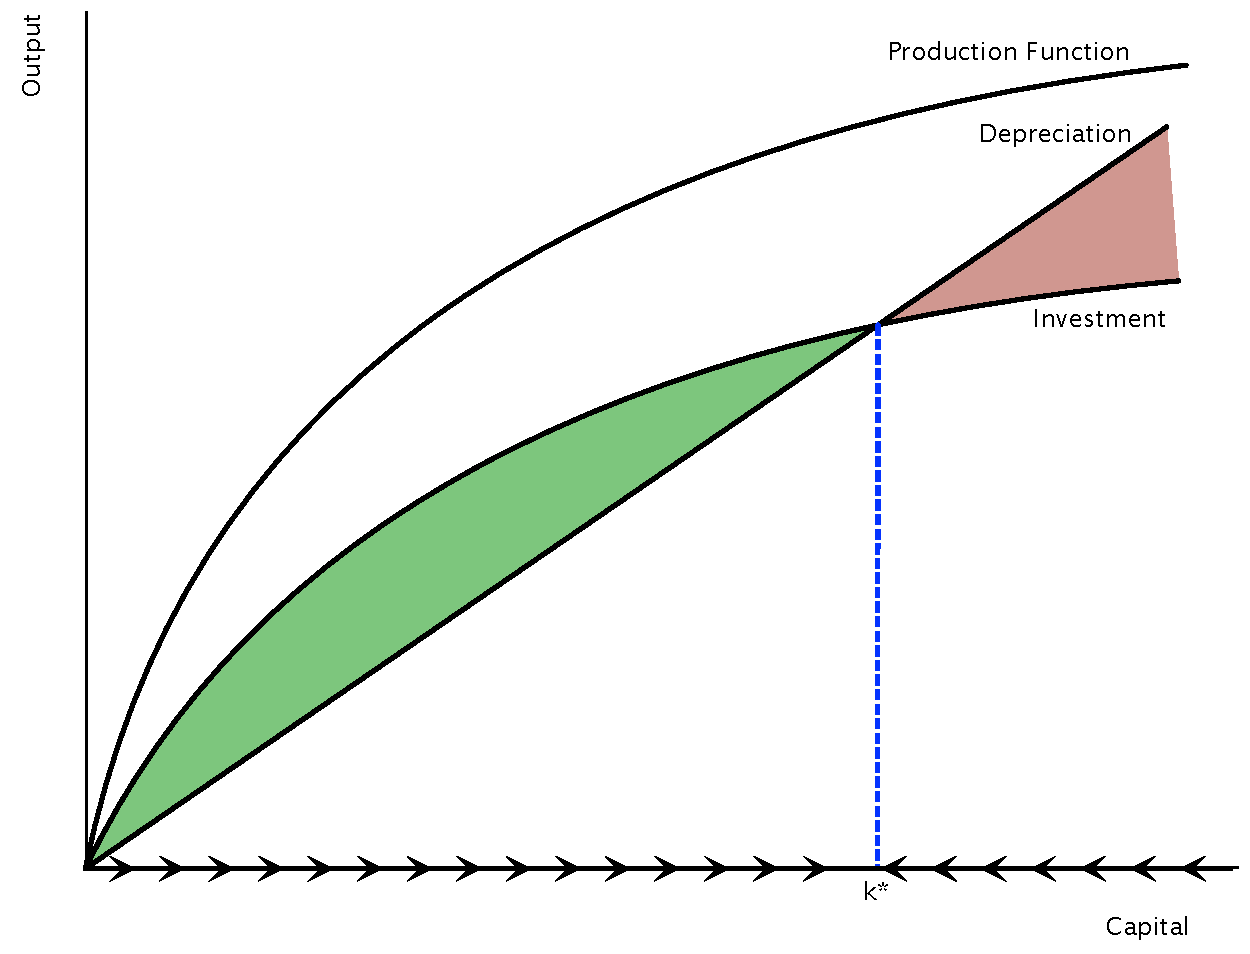
\includegraphics[scale=.35]{plot84.pdf}
	\caption{Capital Accumulation}
\end{figure}
\end{frame}

\section{The Steady State}

\begin{frame}{The Solow Model}
\begin{itemize}
	\item An economy's \textbf{steady state} is an equilibrium path in which $k_t = k^{*}$ for all $t$. 
	\begin{itemize}
	\item If $i>d$, then $k$ and $y$ are \dd{increasing}. 
	\item If $i<d$, then $k$ and $y$ are \dd{decreasing}. 
	\item Finally, if $i = d$, then $k$, $y$, $i$, $c$, $d$ are all \dd{constant}.
\end{itemize}
	\item Thus, the condition that must hold is that investment and depreciation must be \dd{equal}.
\end{itemize}
\end{frame}

\begin{frame}{The Solow Model}
\begin{figure}[H]
	\centering
	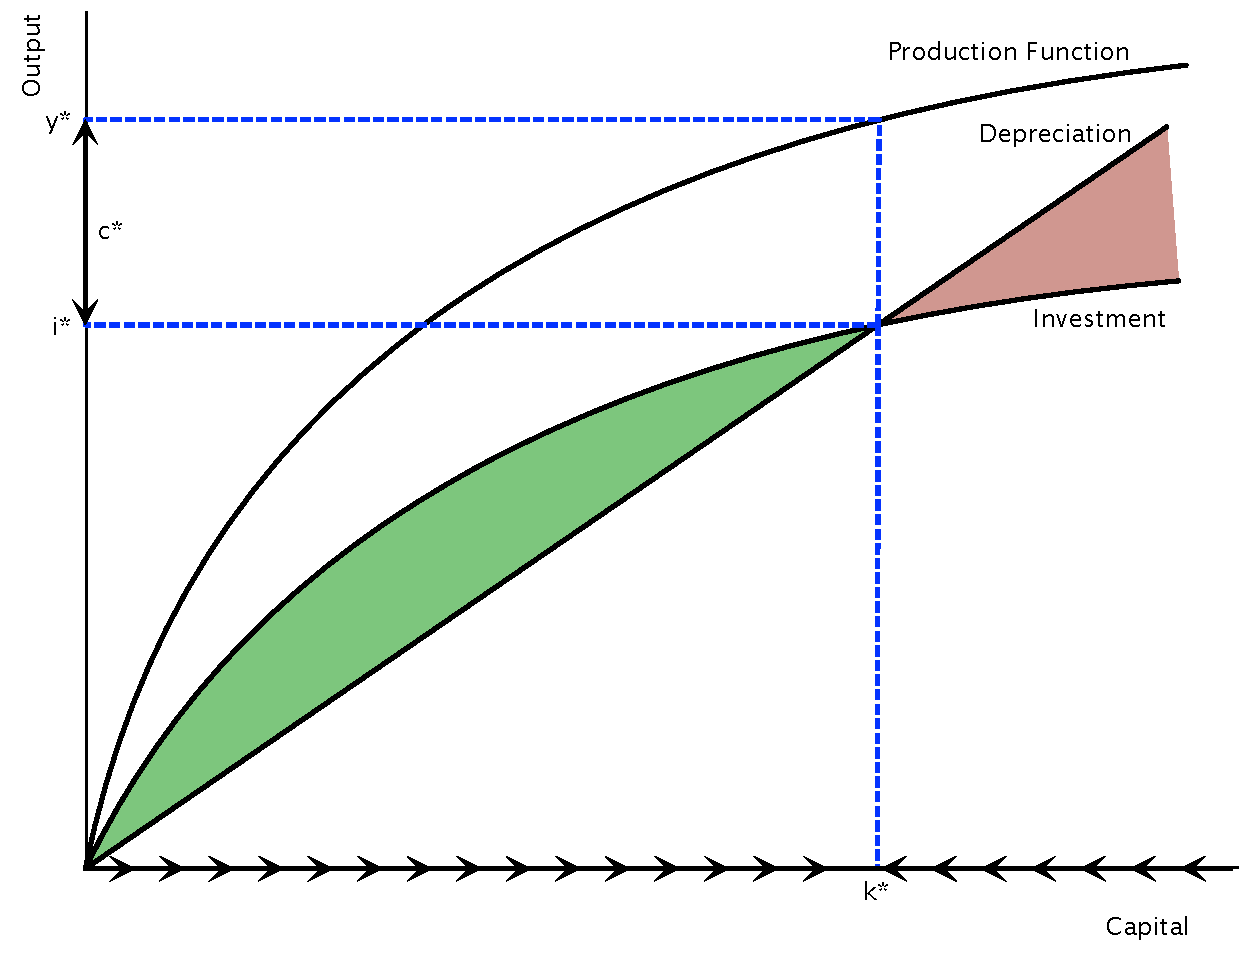
\includegraphics[scale=.35]{plot85.pdf}
	\caption{The Steady State}
\end{figure}
\end{frame}

\begin{frame}{The Solow Model}
\begin{itemize}
	\item As a country approaches its steady state, the growth rate of capital and output \dd{slows} due to diminishing returns. 
	\item In the steady state, real GDP is constant each period and thus economic growth is \dd{zero}. Because of diminishing returns, capital accumulation alone cannot lead to sustained long-run growth. 
\end{itemize}
\end{frame}

\begin{frame}{The Solow Model}
\begin{exmp} 
	A country has the production function $y = \sqrt{k}$. Assume capital depreciates 10\% every period and the country invests 25\% of their output for next period. What is the steady state level of capital per worker? The steady state level of output per worker? 
\end{exmp}

\ddp{$d = .10k$, $i=.25\sqrt{k}$ \\
	Step 1: Set $i = d$ \pause $\Rightarrow .25\sqrt{k} = .10k$ \\
	Step 2: Solve for $k^*$: \pause $\Rightarrow (.10k)^2 = (.25\sqrt{k})^2 \Rightarrow .01k^2 = .0625k \Rightarrow k^* = .0625/.01 = 6.25$ \\
	Step 3: Find $y^*$ \pause $\Rightarrow y^* = \sqrt{6.25} = 2.5$.}
\end{frame}

\begin{frame}{The Solow Model}
\begin{exmp}
	Suppose this country has reached its steady state. How much capital per worker depreciates each period? How much output is invested? How much output is consumed? 
\end{exmp} 
\ddp{\pause $d^* = \delta k^* = .10(6.25) = .625$ \\
	\pause $i^* = sy^* = .25(2.5) = .625$ \\
	\pause $c^* = y^* - i^* = (1-s)y^* = .75(2.5) = 1.875$.}
\end{frame}

\section{Comparative Statics}

\begin{frame}{The Solow Model}
\begin{itemize}
	\item Comparative statics: What happens to the steady state when we change exogenous variables in the model?
	
	\begin{figure}[H]
		\centering
		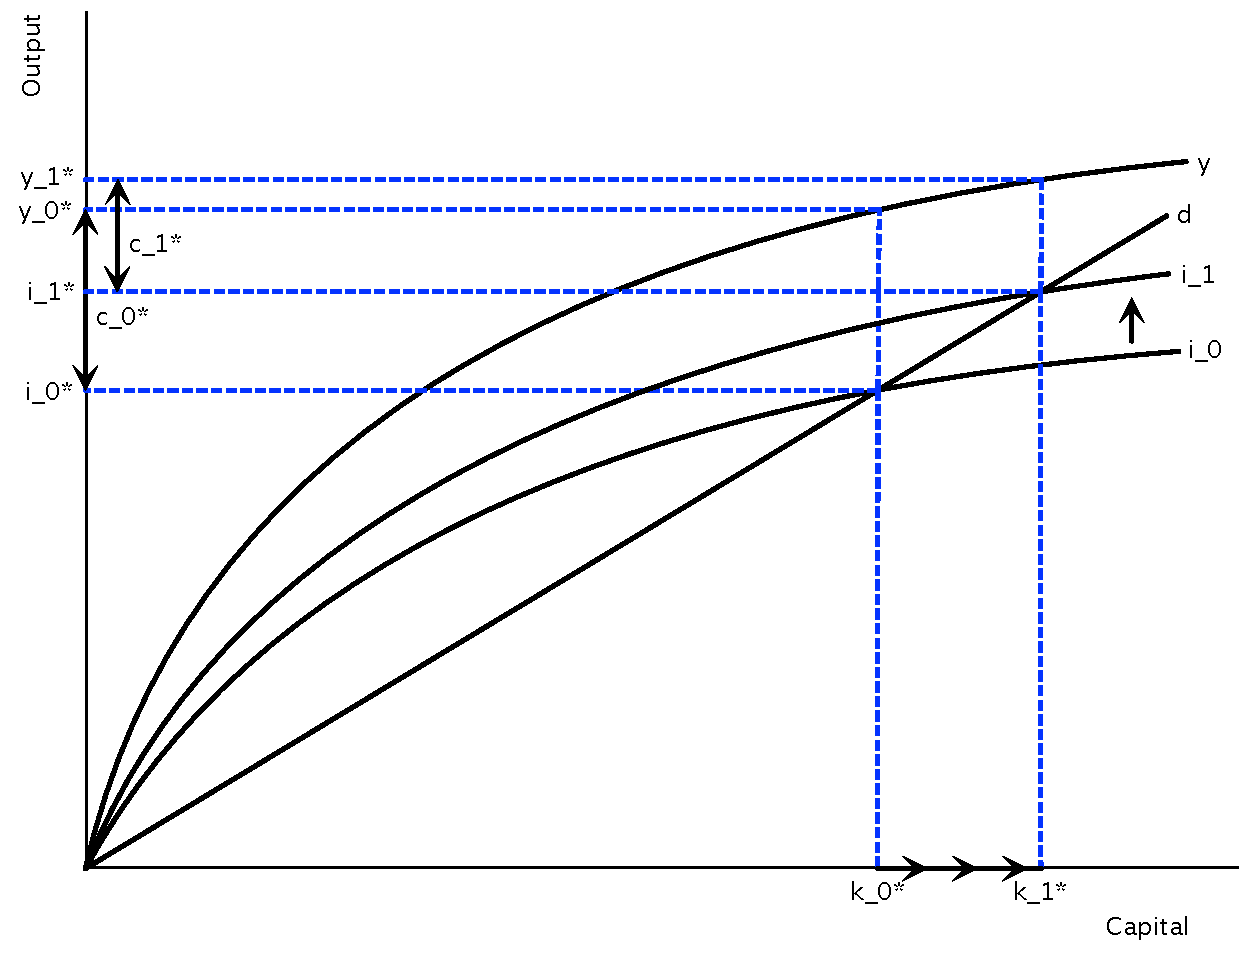
\includegraphics[scale=.35]{plot86.pdf}
		\caption{An Increase in the Savings Rate}
	\end{figure}

\end{itemize}
\end{frame}

\begin{frame}{The Solow Model}
\begin{itemize}
	\item An increase in the savings rate will:
	\begin{enumerate}
		\item Immediately increase investment and decrease consumption.
		\item Lead to a higher steady-state level of capital, output, and investment.
		\item The steady-state level of consumption may increase or decrease depending on the savings rate.
	\end{enumerate}
	\item A decrease in the savings rate will have the opposite effect on 1 \& 2, and the same effect on 3.
\end{itemize}
\end{frame}

\begin{frame}[b]{The Solow Model}
\begin{figure}[H]
	\centering
	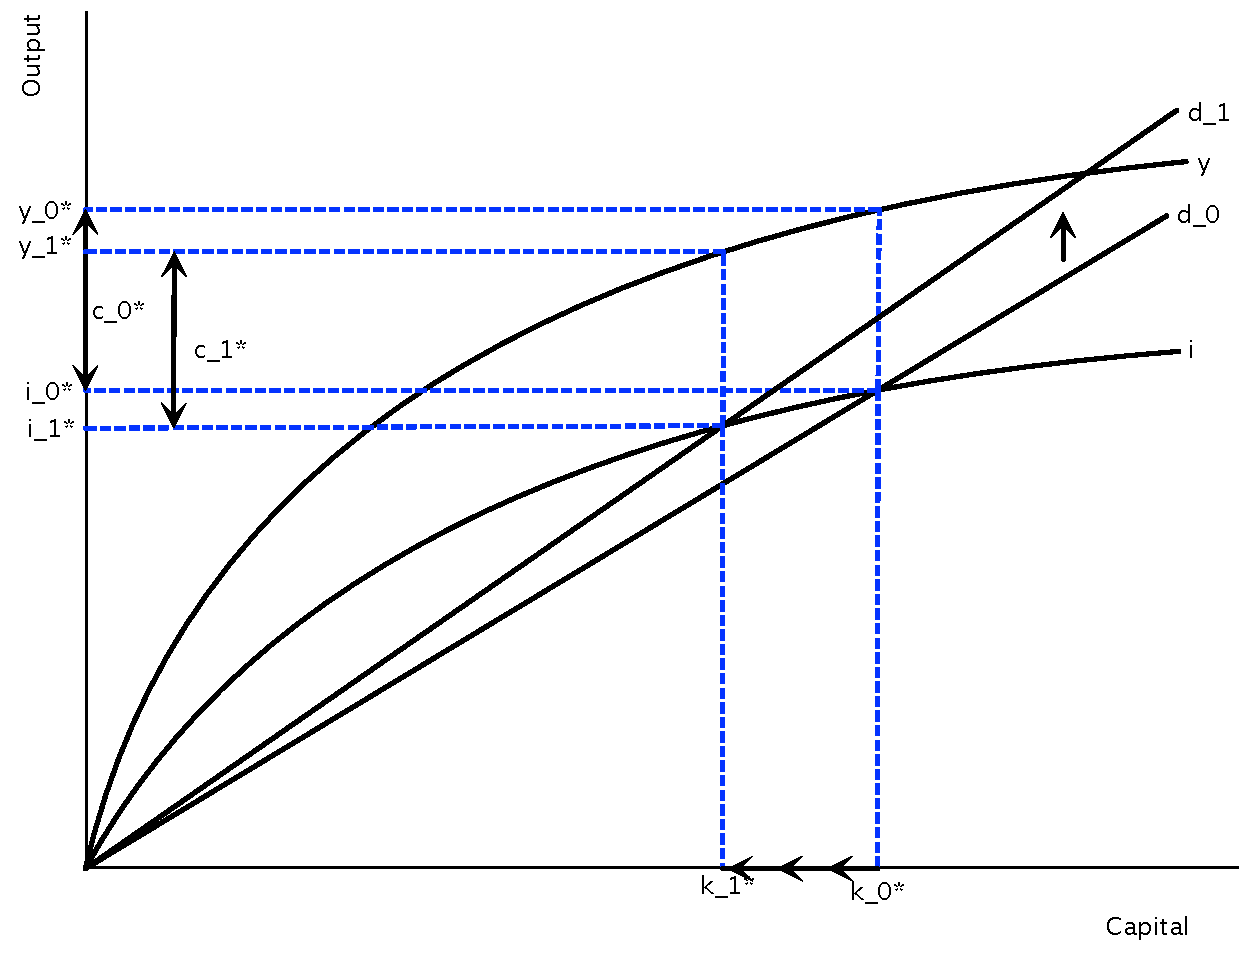
\includegraphics[scale=.35]{plot87.pdf}
	\caption{A Change in the Depreciation Rate}
\end{figure}
\end{frame}

\begin{frame}{The Solow Model}
\begin{itemize}
	\item An increase in the depreciation rate will:
	\begin{enumerate}
		\item Have no impact on current investment and consumption.
		\item Lead to a lower steady-state level of capital, output, investment, and consumption
	\end{enumerate}
	\item A decrease in the depreciation rate will have the opposite effect on 2, and the same effect on 1.
\end{itemize}
\end{frame}

\section{Extensions}

\begin{frame}{The Solow Model}
\begin{itemize}
	\item We model available production technology in the Solow Model by writing $y = A \times f(k)$.
	\item $A$ is a measure of \dd{productivity} and has a \dd{multiplicative} effect.
	\item Technological advances allow countries to sustain growth in the long run. This type of growth is referred to as \dd{cutting-edge} growth.
\end{itemize}
\end{frame}

\begin{frame}{The Solow Model}
\begin{exmp}
	A country has the production function $y = 2\sqrt{k} $. Assume capital depreciates 10\% every period and the country invests 25\% of their output for next period. What is the steady state level of capital per worker? The steady state level of output?
\end{exmp} 
\end{frame}

\begin{frame}[b]{The Solow Model}
\begin{figure}[H]
	\centering
	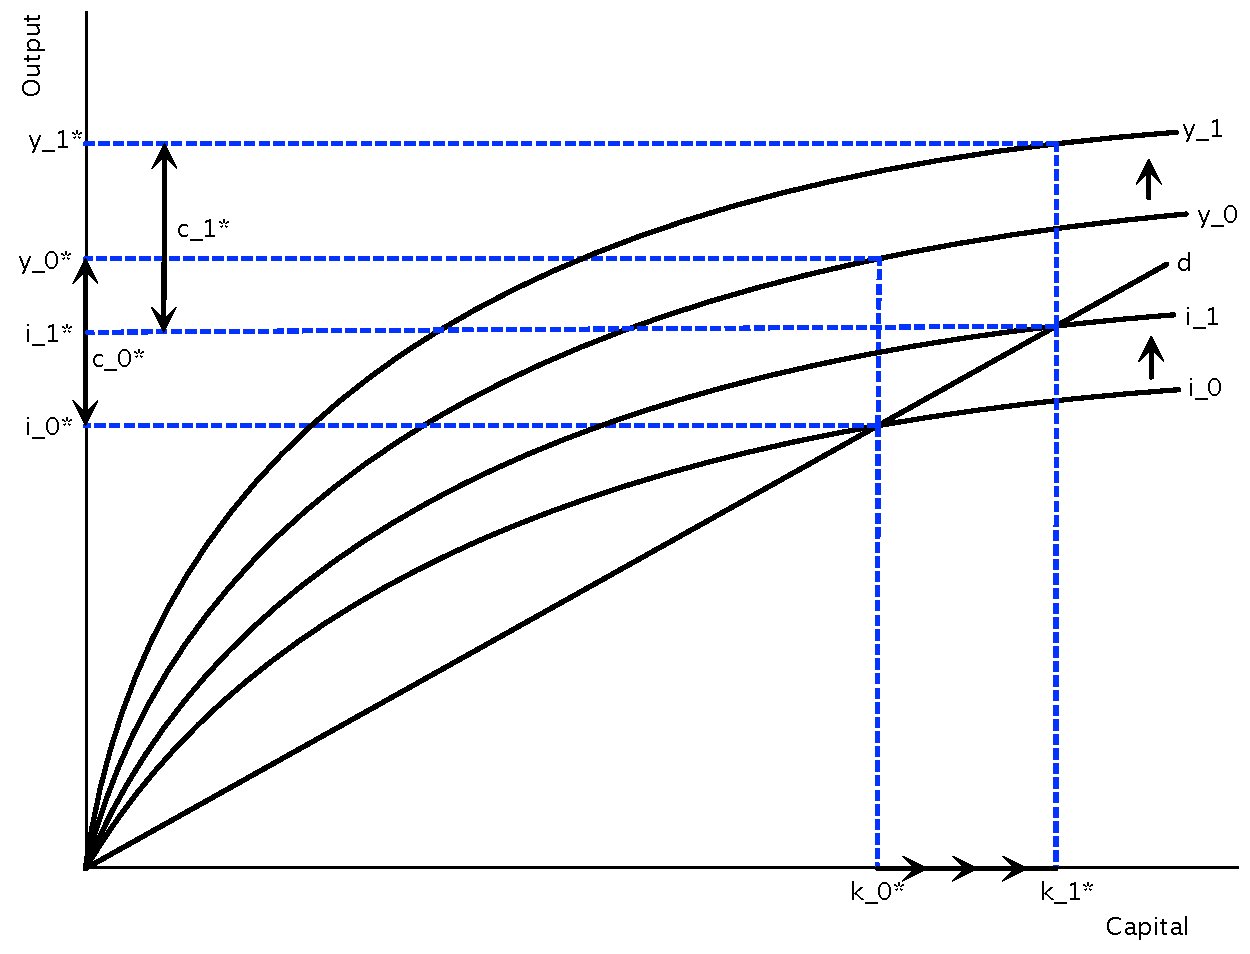
\includegraphics[scale=.35]{plot88.pdf}
	\caption{A Change in Technology}
\end{figure}

\end{frame}

\begin{frame}{The Solow Model}
\begin{itemize}
	\item Assumption: Population and the labor force grow at a constant rate $n$. 
	\item Now, capital per worker decreases each period not only through depreciation, but also because it is spread out over more workers. This is referred to as \dd{capital dilution}. 
	\item Thus, the depreciation of capital per worker every period is now written as $d_t = (n + \delta)k_t$.
\end{itemize}
\end{frame}

\begin{frame}{The Solow Model}
\begin{exmp} 
	A country has the production function $y = \sqrt{k}$. Assume capital depreciates 10\% every period and the country invests 25\% of their output for next period. Moreover, the population grows 2\% every year. What is the steady state level of capital per worker? The steady state level of output?
\end{exmp}

\end{frame}

\begin{frame}{Readings and Assignments}
\begin{itemize}
	\item Today: Mankiw Ch. 26
	\item Next time: Mankiw Ch. 28
	\item Problem Set 5, section 3
\end{itemize}
\end{frame}

\end{document}